\subsection*{\textbf{\RQfive}}

\vspace{3mm}	
\noindent\textbf{77\% (\nicefrac{338}{441}) of participants agree with the statement that CI shortens the delivery time of merged PRs.}
In question \#12 of our survey, we ask participants to express the extent to which they agree with the following statement: ``the adoption of CI shortens the time to deliver merged PRs to end users.'' Most of our participants (77\%, \nicefrac{338}{441}) agree with the statement, while 16\% (\nicefrac{72}{441}) are neutral, and 7\% (\nicefrac{31}{441}) disagree or strongly disagree with the statement (see Figure \ref{fig:developer_perception_about_impact_of_ci_on_delivery_time}). However, it is not clear whether these latter participants perceive CI as not having any influence on the delivery time of merged PRs or whether they perceive CI as having a negative influence on the delivery time of merged PRs.

\begin{figure}[h!]
	% Use the relevant command to insert your figure file.
	% For example, with the graphicx package use
	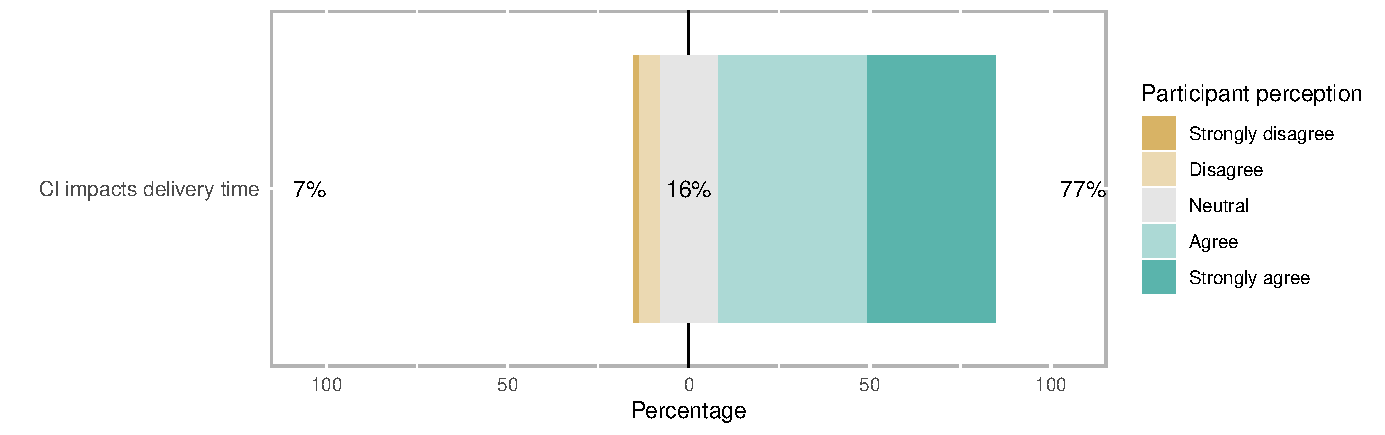
\includegraphics[height=4cm, width=12cm]{developers_accordance_on_the_impact_of_ci_on_delivery_time.pdf}
	% figure caption is below the figure
	\caption{Developer's perception about the influence of continuous integration on the delivery time of merged pull requests (\textit{Question \#12}).}
	\label{fig:developer_perception_about_impact_of_ci_on_delivery_time}       % Give a unique label
\end{figure}

After analyzing our participants' responses, the influence of CI on the delivery time of merged PRs was captured through the following themes: \textit{release process}, \textit{project quality}, and \textit{automation}. The description and examples of mentions for each theme are presented in the following. Additionally, Table \ref{tab:frequency_citation_CI_factors_impact} shows the frequency of mentions for each code and theme related to how CI may influence the delivery time of merged PRs. 

% Table generated by Excel2LaTeX from sheet 'IMPACT OF CI ON DELIVERY TIME'
\begin{table}
	\centering
	\caption{Frequency of mentions in participants' responses for each code and theme related to how CI may influence the delivery time of merged PRs.}
	\begin{tabular}{cp{10.75em}cc}
		\hline
		\multirow{2}[4]{*}{\textbf{Theme}} & \multirow{2}[4]{*}{\textbf{Code}} & \multicolumn{2}{c}{\textbf{Frequency}} \bigstrut\\
		\cline{3-4}          & \multicolumn{1}{c}{} & \multicolumn{1}{p{5.415em}}{\textbf{Frequency per code}} & \multicolumn{1}{p{5.585em}}{\textbf{Frequency per theme}} \bigstrut\\
		\hline
		\multirow{7}[14]{*}{\textbf{Automation}} & Automated testing & 39    & \multirow{7}[14]{*}{99} \bigstrut\\
		\cline{2-3}          & Earlier feedback & 24    &  \bigstrut\\
		\cline{2-3}          & Reduced testing time & 10    &  \bigstrut\\
		\cline{2-3}          & Reduced burden on reviewers & 9     &  \bigstrut\\
		\cline{2-3}          & Automated building & 7     &  \bigstrut\\
		\cline{2-3}          & Less manual work & 6     &  \bigstrut\\
		\cline{2-3}          & Improved automation & 4     &  \bigstrut\\
		\hline
		\multirow{5}[10]{*}{\textbf{Project quality}} & Code quality & 14    & \multirow{5}[10]{*}{130} \bigstrut\\
		\cline{2-3}          & Code stability & 23    &  \bigstrut\\
		\cline{2-3}          & Higher test coverage & 6     &  \bigstrut\\
		\cline{2-3}          & Better confidence & 83    &  \bigstrut\\
		\cline{2-3}          & Reduced regression risk & 4     &  \bigstrut\\
		\hline
		\multicolumn{1}{c}{\multirow{3}[6]{*}{\textbf{Release process}}} & Faster release cycle & 29    & \multirow{3}[6]{*}{49} \bigstrut\\
		\cline{2-3}          & Automated deployment & 17    &  \bigstrut\\
		\cline{2-3}          & Smaller release & 3     &  \bigstrut\\
		\hline
	\end{tabular}%
	\label{tab:frequency_citation_CI_factors_impact}%
\end{table}%

\vspace{0.6mm}
\noindent\textbf{Release process.\textsuperscript{(49)}} Several responses to our questionnaire indicate that the adoption of CI influences the delivery time of merged PRs because CI promotes \textit{faster release cycles}.\textsuperscript{(29)} For instance, 
%C420 states that \textit{``CI releases are smaller, well tested, and generally frequent and low risk,''}, whereas 
C346 declares that \textit{``Good use of CI could help in faster release cycle, because you can be more confident in shipping something that works.''} Some practitioners of CI \citep{goodman2008s} have claimed that some benefits of using CI are the improved release frequency and predictability. However, our quantitative study ($RQ2$) does not support such a claim. We do not observe a significant difference in release frequency \textit{after} the adoption of a CI service (e.g., \textsc{TravisCI}) for the studied projects. Furthermore, we found that \textit{after} the adoption of \textsc{TravisCI}, projects delivered 3.43 times more PRs per release than \textit{before} the adoption of \textsc{TravisCI}. We observe that although the release frequency was not significantly affected by the adoption of a CI service, projects process substantially more PRs per release than \textit{before} the adoption of \textsc{TravisCI}.
Furthermore, \textit{automated deployment}\textsuperscript{(17)} can be another step in the adoption of CI which helps projects to rapidly deliver software changes to end users \citep{Humble2010-ca}. 
Automated deployment refers to the process of making developers' code available to end users automatically \citep{rahman2015synthesizing}.  C347 explains that \textit{``CI is the only way to automate deployment, thus speeding up customer delivery''}.
 Finally, developers also mentioned \textit{smaller releases}\textsuperscript{(3)} as an influencing factor of CI on the delivery time of merged PRs. For instance, C076 states that it \textit{``makes sense for the releases to be smaller and more frequent as a project reaches a level of stability.''} 

\vspace{0.6mm}
\noindent\textbf{Project Quality.\textsuperscript{(130)}} This is the theme most mentioned by our participants. According to participants, CI influences the delivery time of merged PRs by increasing \textit{code quality},\textsuperscript{(14)} providing \textit{code stability},\textsuperscript{(23)} and reducing \textit{regression risks}.\textsuperscript{(4)} For example, C280 states that CI promotes a \textit{``much better quality of contributions and therefore much shorter release cycles.''} Also, CI influences code stability, as declared by C270: \textit{``it makes the required time to deliver shorter because the maintainer can be relatively sure the change does not break other use cases.''} 
According to \cite{Vasilescu2015-tn}, core developers using CI can discover more bugs than developers in projects not using CI. \textit{Better quality confidence}\textsuperscript{(83)} is the most mentioned code when it comes to the adoption of CI. According to participants, the delivery time of merged PRs is positively influenced by CI because 
\textit{``it's much easier to trust a PR that was built and tested at a CI environment than having to do everything manually on my own machine''} (C361). This trust in CI is also related to a \textit{higher test coverage}.\textsuperscript{(6)} For instance, C151 states that
\textit{``CI requires a good test suite, which gives confidence in the correctness of the project.''} Indeed, poor test coverage may make successful builds misleading~\citep{felidre2019continuous} (i.e., the builds may still contain unidentified bugs). 

\vspace{06.mm}
\noindent\textbf{Automation.\textsuperscript{(99)}} 
According to our participants, CI also influences the delivery time of merged PRs by \textit{improving automation}.\textsuperscript{(4)} Automation is a key aspect of CI. Projects implementing proper CI must at least automate their build and testing processes. Automation leads to \textit{less manual work},\textsuperscript{(6)} as explained by C203 when stating that \textit{``Yes, the amount of manual work involved in a release is much less when you use CI.''}	
The \textit{automated testing}\textsuperscript{(39)} code is mentioned several times as influencing the delivery time of merged PRs, which is in accordance with the study by \cite{rahman2015synthesizing}.
For example, C361 states that \textit{``I worked on the Bokeh project both before and after the full integration of \textsc{TravisCI}. Previously, major releases took months of planning due to a lack of manpower needed for running tests. With the adoption of CI, new versions can be released semi-monthly thanks to CI greatly reducing the number of man-hours needed for testing.''} 

The automated test execution provides \textit{earlier feedback},\textsuperscript{(24)} which is also recurrently mentioned by our participants. For instance, C439 states that \textit{``early errors are identified by CI, so it facilitates the delivery process.''} 
Also according to our participants, CI contributes to a \textit{reduced testing time}.\textsuperscript{(10)} C062 states that \textit{``when you have CI (+ a strong test suite) you can in some cases shorten a lot the manual test of that bug fix, or in some cases even skip it entirely (when the fix is simple enough).''} Finally, it was also mentioned that CI contributes to a \textit{reduced burden on reviewers}.\textsuperscript{(9)} For instance, C026 declares that \textit{``relying on reviewers to build to test will increase time to ship massively and will be a drain on the already scarce resource of reviewers.''} This observation is interesting as it may explain our results in $RQ2$ related to the higher number of PRs delivered per release (see Section~\ref{sec_quantitative_study_results}), i.e., as there is less burden to reviewers, they have more capacity to review PRs that, otherwise, would have waited longer in the delivering queue. Previous studies observed that there is less discussion in PRs \textit{after} the adoption of CI \citep{cassee2020silent}, which could also save reviewers' time. The use of CI automates several tasks in software development (i.e., build and test), thus saving time from maintainers, so they can focus on the content of the proposed software changes and launch software releases. Indeed, several participants stated that \textit{automated building}\textsuperscript{(7)} quickens the delivery time of merged PRs. For instance, C400 declares that \textit{``it [automated building] reduced the required time [to deliver] since CI built code, run tests etc.''} 

\begin{figure}[hbt!]
	% Use the relevant command to insert your figure file.
	% For example, with the graphicx package use
	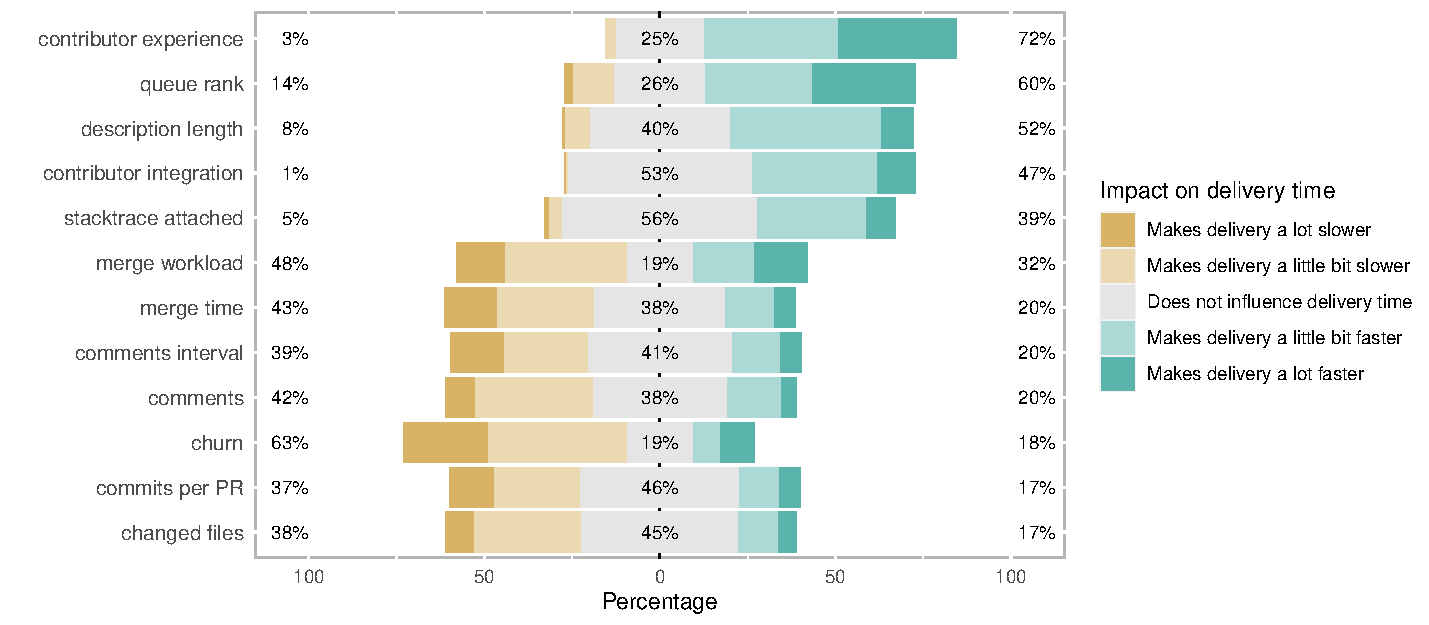
\includegraphics[height=6cm, width=12cm]{factors_impact_on_delivery_time.pdf}
	% figure caption is below the figure
	\caption{Developers' perception about factors' impact on the delivery time of merged PRs (\textit{Question \#12}).}
	\label{fig:factors_impact_on_delivery_time}       % Give a unique label
\end{figure}

\vspace{06.mm}
\noindent\textbf{According to our participants, \textit{PR churn} and the number of PRs waiting to be merged (\textit{merge workload}) are the most important variables of our models in Study I}. 
In question \#12, we request our participants to rate the degree to which 12 variables used in our regression models (see $RQ3$, Tables \ref{tab_explanatory_variables_1} and \ref{tab_explanatory_variables_2}) may influence the delivery time of merged PRs. We present the following variables: (i) a number that represents the moment at which a PR is merged compared to other merged PRs within the release cycle (queue rank); (ii) contributor integration; (iii) stack-trace attached; (iv) description size; (v) contributor experience; (vi) merge workload; (vii) changed files; (viii) churn; (ix) merge time; (x) number of commits per PR; (xi) number of comments; and (xii) interval of comments. 

Our participants were invited to rate their perception regarding the impact of each above-mentioned variable on a 5-point Likert scale. The options were the following: (i) makes delivery a lot slower; (ii) makes delivery a little bit slower; (iii) does not influence the delivery time; (iv) makes delivery a little bit faster; and (v) makes delivery a lot faster.
Figure \ref{fig:factors_impact_on_delivery_time} shows the perception of participants regarding the influence of each variable on the delivery time of merged PRs. Figure \ref{fig:factors_impact_on_delivery_time_heating} shows the frequency of each rating per variable. The lower the percentage of \textit{``does not influence delivery time,''} the higher the perceived influence of a variable on the delivery time of merged PRs.

The variables that are most rated as having influence on the delivery time are \textit{churn} and \textit{merge workload}. This finding is partially in agreement with our regression models (see $RQ3$). The \textit{merge workload} is also one of the most influential variables in our models. According to our regression models, the higher the merge workload the higher the delivery time of merged PRs. This is in agreement with the perception of 81\% of participants of our survey. 
The influence of \textit{merge workload} is explained by 
C093, when they mention that a longer delivery time can be due to \textit{``not enough developers and too many pull requests \& issues to manage"}. Contrasting our models, participants rated \textit{PR churn} as one of the most influential codes on delivery time. When asked about examples of merged PRs that took long to be delivered, 
C109 mentioned PRs that have a \textit{``big change for a core function''}.
However, our regression models ($RQ3$) do not rate \textit{code churn} as an influential variable to explain delivery time. Another agreement between our models and participants is that 73.8\% of participants rate \textit{queue rank} as influential to explain the delivery time of merged PRs. This corroborates the results from $RQ3$, which reveals that \textit{queue rank} is influential when explaining delivery time. 

Although the responses from participants confirm the influence of certain variables used in our regression models ($RQ3$), in Figure \ref{fig:factors_impact_on_delivery_time_heating}, we observe that the option \textit{``Does not influence delivery time"} is frequently chosen for many other variables. 6 out of 12 variables (\textit{stacktrace attached}, \textit{description length}, \textit{contributor integration}, \textit{commits per PR}, \textit{comments interval} and \textit{changed files}) were ranked above 40\% (2 being over 50\%), which means that a substantial number of participants is skeptical regarding the influence of such variables on delivery time. This finding supports our regression model's results, except for the contributor integration metric. The contributor integration is the third most influential variable in our models for time periods \textit{before} and \textit{after} the adoption of \textsc{TravisCI}. Our models suggest that if a contributor has their prior PR delivered quickly, their future PRs are more likely to be delivered quickly.


\begin{figure}[tbh]
	% Use the relevant command to insert your figure file.
	% For example, with the graphicx package use
	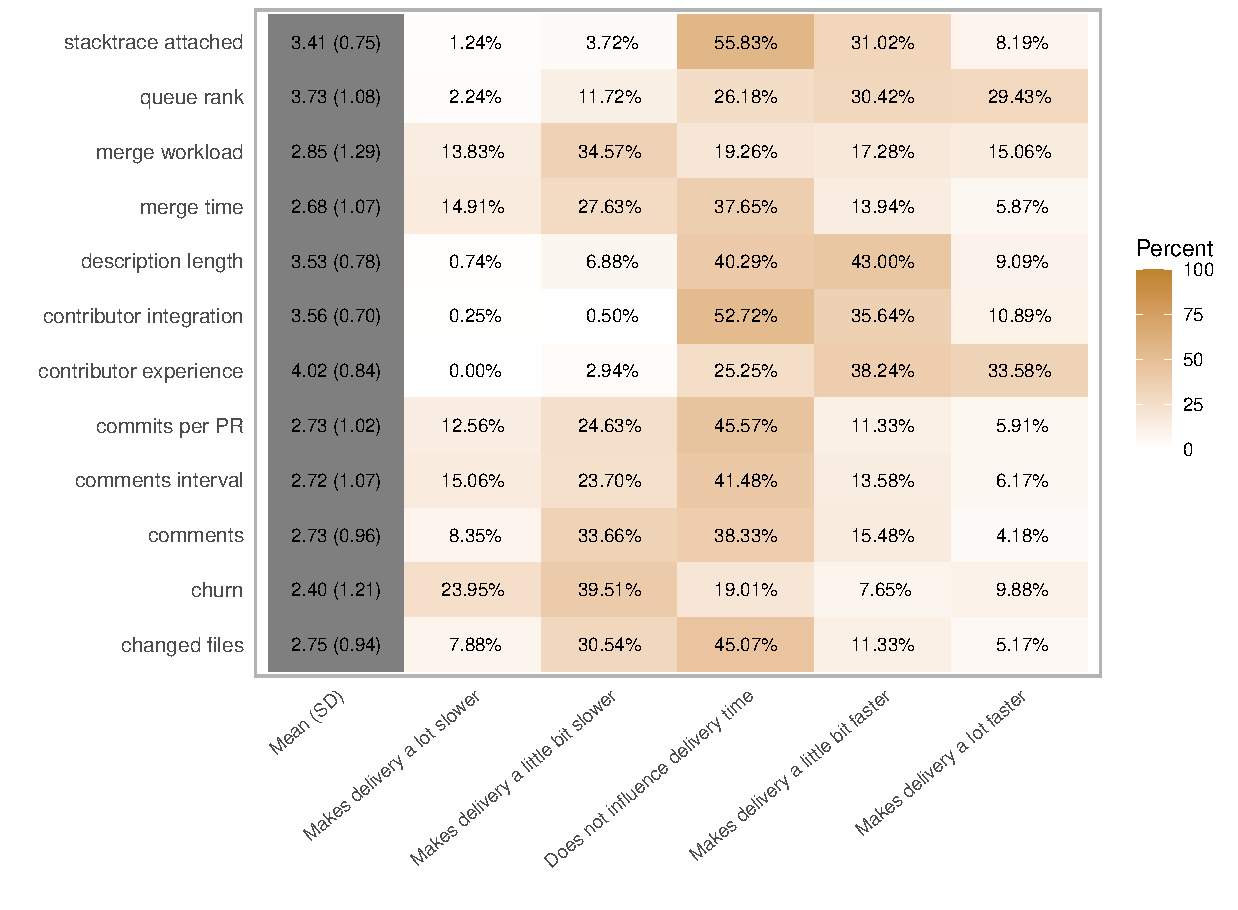
\includegraphics[height=8cm, width=12cm]{factors_impact_on_delivery_time_heating.pdf}
	% figure caption is below the figure
	\caption{Rating of codes related to delivery time of merged PRs (\textit{Question \#13}).}
	\label{fig:factors_impact_on_delivery_time_heating}       % Give a unique label
\end{figure}

\vspace{06.mm}
\noindent\textbf{When presented with the median delivery time of merged PRs \textit{before} and \textit{after} the adoption of \textsc{TravisCI}, 42.9\% (\nicefrac{140}{326}) of participants state that \textsc{TravisCI} has little influence on the delivery time, attributing the change
in delivery time to other unrelated factors.} 
According to responses to Question \#26 of our survey, 
42.9\% of participants attribute the delivery time of PRs to other factors not directly related to the adoption of \textsc{TravisCI} (i.e., project maintenance, release strategy, and PR characteristics).
As an example, we observe that the median delivery time of PRs in the \textit{rails/rails} project increased from 120 to 184 days \textit{after} the adoption of \textsc{TravisCI}. However, according to 13 participants of the \textit{rails/rails} project, \textit{``this is definitely not related to CI. \textit{rails/rails} has its own release schedules''} (C063). Furthermore, when we presented the data for participants of the \textit{ansible/ansible} project, where the median delivery time increased from 36 to 121 days (\textit{after} the adoption of \textsc{TravisCI}), C355 explained that \textit{``all depends on the project owners decision when to release.''} Additionally, in $RQ5$, we further discuss the factors that participants argue to not being directly related to CI, but can influence the delivery time of merged PRs.

\begin{center}
    \begin{tabular}{|p{.96\columnwidth}|}
        \hline
        \textbf{Summary:}
        \textit{The general perception is that CI influences the delivery time by improving \textit{automation}, the \textit{release process}, and the \textit{project quality}. Furthermore, \textit{code churn} and \textit{merge workload} are the variables with the highest perceived influence on the delivery time of merged PRs.  
        However, when showing specific project data to the respective participants, 42.9\% of participants are skeptical regarding the influence of CI on the delivery time of the merged PRs.} \\
        \textbf{Implications:}
        \textit{Our participants consider that the key benefit of CI is to improve the mechanisms by which project contributions are processed (e.g., facilitating decisions related to PR submissions), without compromising the quality or overloading the reviewers and maintainers of the projects.}
        \\
        \hline
    \end{tabular}
\end{center}